\documentclass{article}
\usepackage{amssymb}
\usepackage{amsmath}
\textheight20cm 

\usepackage{verbatim}
\usepackage[dvips]{color}
\usepackage{amsfonts}
\usepackage{graphicx}
\usepackage{latexsym}
\usepackage{rotating}
\usepackage{url}
\usepackage{xspace}
\usepackage[breaklinks=true,colorlinks,citecolor=blue]{hyperref}



\newcommand{\Q}{{\mathbb Q}}
\newcommand{\OO}{{\mathbb O}}
\newcommand{\Z}{{\mathbb Z}}
\newcommand{\R}{{\mathbb R}}
\newcommand{\N}{{\mathbb N}}
\newcommand{\X}{{\mathbb X}}
\newcommand{\latte}{{\tt LattE}\xspace}
\newcommand{\latteInt}{{\tt LattE integrale}\xspace}
\newcommand{\latteMac}{{\tt LattE macchiato}\xspace}
\newcommand{\latteV}{v1.5}
\newcommand{\vinci}{{\tt Vinci}\xspace}
\newcommand{\maple}{{\tt Maple}\xspace}
\newcommand{\cdd}{{\tt CDD}\xspace}
\newcommand{\fourtitwo}{{\tt 4ti2}\xspace}
\newcommand{\cubpack}{{\tt CUBPACK}\xspace}
\newcommand{\example}{{\bf Example:\space}}


\DeclareMathOperator{\vol}{vol}     %%% Denotes volume
\DeclareMathOperator{\Res}{Res}  %% Residue
\renewcommand\d{\,\mathrm{d}}
\newtheorem{theorem}{Theorem}

\setlength{\parindent}{0pt}
\setlength{\parskip}{2ex plus 0.4ex minus 0.4ex}

\title{A User's Guide for {\tt LattE integrale} \latteV \\ (Linux Release) 
\footnote{Research supported by NSF grants DMS-0309694, NSF grants
DMS-0073815, DMS-0914107 and DMS-0914873.
Most of the students were supported by those
grants and by summer fellowships provided through the UC Davis VIGRE grants
DMS-0135345 and DMS-0636297. $\copyright$ 
Department of Mathematics, University of California, Davis, 2011. This
software is released under the GNU license agreement}
\\ 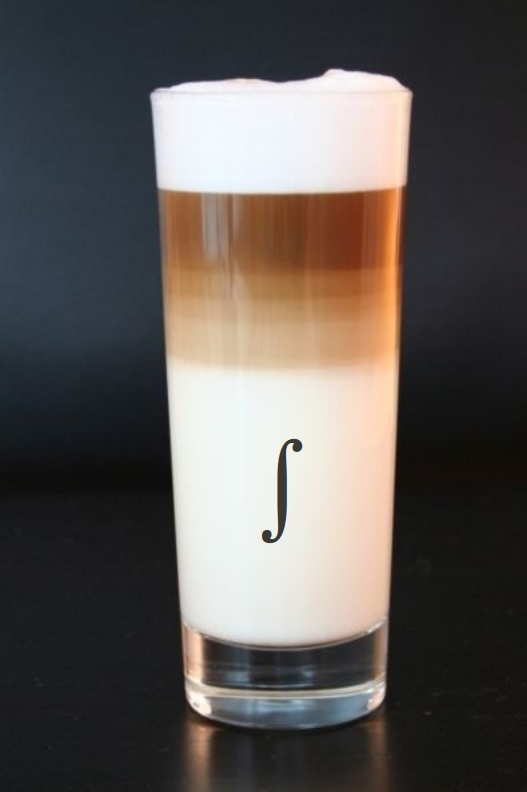
\includegraphics[width=0.25\textwidth]{latte-integrale.jpg}
}%close title brace

\author{Jes\'us A. De Loera \and
Brandon Dutra \and
Matthias K\"oppe \and 
Stanislav Moreinis \and
Gregory Pinto \and
Jianqiu Wu \and
}
 

 
 \date{July 2011}

\begin{document}

\maketitle{}

\newpage

\tableofcontents

\newpage

\section{Introduction}

\subsection{What is {\tt LattE}?} \label{intro}

The name ``{\tt LattE}'' is an abbreviation for ``{\bf Latt}ice point 
{\bf E}numeration.'' \latte was developed in 2001 to count lattice points contained in 
convex polyhedra defined by linear equations and inequalities with 
integer coefficients. The polyhedra can be of any (reasonably small) 
dimension. In 2007, {\tt LattE macchiato} was released and contained many 
algorithmic improvements. The newest edition, {\tt LattE integrale}, developed
in 2010 can compute integrals of polynomials and volumes of rational polytopes. 
All these algorithms run in polynomial
time for fixed dimension. To
learn more about the exact details of our implementation for lattice point enumeration, the interested reader can consult 
\cite{koeppe:irrational-barvinok, latte1} and the references listed therein. 
For learning the algorithmic details of integration, see \cite{howToIntegratePolynomialSimplex, latte-integrale-paper}. Here we
give a rather short description of the mathematical objects used by
{\tt LattE}. Note that all our computations are done over the integers or the rationals {\emph exactly}.
\latte cannot compute with floating-point numbers. 

\subsubsection{Counting lattice points: Barvinok's Rational Functions}

Given a convex polyhedron $P = \{u\in\R^d:Au\leq b\}$, where $A$ and
$b$ are integral, the fundamental object that we compute is a short 
representation of the infinite power series:
\[
f(P;x) \quad = \sum_{\alpha\in P\cap\Z^d} x_1^{\alpha_1}
x_2^{\alpha_2} \ldots x_d^{\alpha_d}.
\]
Here each lattice point is given by one monomial. Note that this can be 
a rather long sum, in fact for a polyhedral cone it can be infinite, but 
the good news is that it admits short representations.

\example Let $P$ be the quadrangle with vertices 
$V_1=(0,0)$, $V_2=(5,0)$, $V_3=(4,2)$, and $V_4=(0,2)$, see Figure \ref{fig:quadrangle}.

\begin{figure}[thb]
	\centering
	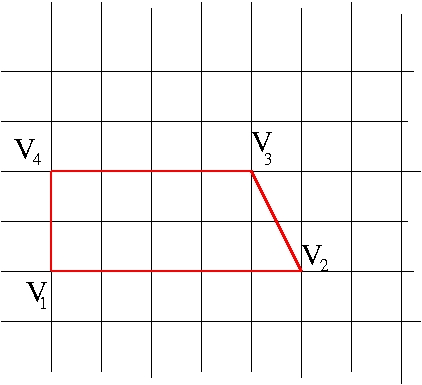
\includegraphics[width=0.7\textwidth]{examplebrion.jpg}
	\caption{Quadrangle with vertices $V_1=(0,0)$, $V_2=(5,0)$, $V_3=(4,2)$, and $V_4=(0,2)$.}
	\label{fig:quadrangle}
\end{figure}

{\small
\noindent
$f(P;x,y)={x}^{5}+{x}^{4}y+{x}^{4}+{x}^{4}{y}^{2}+y{x}^{3}+{x}^{3}+
{x}^{3}{y}^{2}+y{x}^{2}+{x}^{2}+{x}^{2}{y}^{2}+xy+x+x{y}^{2}+y+1+
{y}^{2}$
}

The fundamental theorem of Barvinok (circa 1993, see \cite{BarviPom})
says that you can write $f(P;x)$ as a sum of short rational functions,
in polynomial time when the dimension of the polyhedron is fixed.
In our running example we easily see that the 16 monomial polynomial
can be written as shorter rational function sum:

\noindent $f(P;x,y)=f(K_{V_1};x,y)+f(K_{V_2};x,y)+f(K_{V_3};x,y)+f(K_{V_4};x,y)$ 

\noindent where 

$f(K_{V_1};x,y)={\frac {1}{\left (1-x\right )\left (1-y\right )}} \quad f(K_{V_2};x,y)=\frac{({x}^{5}+{x}^{4}y)}{ (1-{x}^{-1}) (1-y^2x^{-1})}$

$f(K_{V_3};x,y)=\frac{({x}^{4}{y}^{2}+{x}^{4})}{ (1-{x}^{-1})
(1-xy^{-2})}
 \quad  f(K_{V_4};x,y)=\frac{y^{2}}{(1-{y}^{-1} )(1-x )}$
\vskip .5cm

$ f(P; 1,1)=16$

Counting the lattice points in convex polyhedra is a powerful tool which 
allows many applications in areas such as Combinatorics, Statistics, 
Optimization, and Number Theory. 

Fore details of how the computations are done, see \cite{koeppe:irrational-barvinok, latte1} .

\subsubsection{Integration}

\latteInt has two different integration algorithms for integrating a rational polynomial $p \in \R[x_1, \dots, x_d]$ over a $d$ dimensional rational polytope. The first one, called the triangulation method, triangulates the polytope into simplices and integrates over each simplex. The other method, called the cone decomposition method, integrates over each tangent cone of the polytope. In order to do this, each tangent cone is triangulated into simple cones. This is the main trade off between the two integration algorithms: you can do one (possibly) large triangulation, or (possibly) many small tangent cone triangulations. 

We decompose polynomials into finite sums of powers of linear forms because integrating powers of linear forms can be done in polynomial time \cite{howToIntegratePolynomialSimplex}. A decomposition of a polynomial as a sum of powers of linear forms is known as the polynomial Waring problem.

See \cite{latte-integrale-paper} for a detailed explanation on why the next example gives the correct integral. 

As an example, let us integrate the polynomial $x_1+x_2$ over the unit square with vertices $(0,0), (1,0), (0,1)$ and $(1,1)$. The polynomial is already a power of a linear form so let $\ell = (1,1)$. To integrate $\int (x_1+x_2)^M dx$ over the square, we need to compute
\begin{displaymath}
	\frac{M!}{(M+d)!} |\det(u_1, \dots, u_d)| \frac{(\langle \ell, s \rangle)^{M+d}}{\prod_{i=1}^d  \langle -\ell, u_i \rangle}
\end{displaymath}
at each vertex $s$ where the $u_i$ are the rays from the tangent cone at $s$, and $d$ is the dimension of the polytope.

Vertex $s_1 = (0,0)$: Because $\langle \ell, s_1 \rangle ^{1+2} = 0$ the valuation on this cone is zero.

Vertex $s_2 = (1,1)$: 

\begin{displaymath}
 \frac{M!}{(M+d)!} |\det(u_1, \dots, u_d)| \frac{(2)^{1+2}}{(-1)(-1)} = \frac{1!}{(1+2)!} \times 1 \times 8 = 4/3
\end{displaymath}

Vertex $s_3 = (1,0)$: 
	
\begin{displaymath}
 \frac{M!}{(M+d)!} |\det(u_1, \dots, u_d)| \frac{(1)^{1+2}}{(1)(-1)} = \frac{1!}{(1+2)!} \times 1 \times -1 = -1/6
\end{displaymath}


Vertex $s_4 = (0,1):$ 


\begin{displaymath}
 \frac{M!}{(M+d)!} |\det(u_1, \dots, u_d)| \frac{(1)^{1+2}}{(1)(-1)} = \frac{1!}{(1+2)!} \times 1 \times -1 = -1/6
\end{displaymath}

The integral $\int_{x_1 = 0}^{x_1 = 1}\int_{x_2 = 0}^{x_2 = 1} x_1 +x_2  \d{x_1}\d{x_2} = 0 + 4/3 -1/6 - 1/6 = 1$ as it should be.




\subsection{What can {\tt LattE} compute?}

\latte contains three key executables:
\begin{description}
	\item[count] counts lattice points, computes Ehrhart polynomials and Ehrhart series of polytopes. This executable has replaced {\tt ehrhart}, but {\tt ehrhart} is still included for backwards compatibility.
	\item[integrate] integrates polynomials over polytopes.
	\item[max/minimize] perform linear integer optimization.
\end{description}

The other executables in latte are drivers, converters, and other small utility function described in Section \ref{section:file-descriptions}.

%***********************************************************************************
%***********************************************************************************
%***********************************************************************************
%***********************************************************************************
%***********************************************************************************

\section{Input Files}\label{Input Files}

A polytope can be defined from a list of vertices (a v-representation) or a list of hyperplane inequalities (h-representation) and so \latte can start from either representation in different formats. Here are four common file formats:
\begin{enumerate}
	\item \latte style vertex file
	\item \latte style hyperplane file
	\item \cdd style vertex file
	\item \cdd style hyperplane file
\end{enumerate}

Users of {\tt Polymake} will notice that {\tt Polymake}'s facets and vertices are printed in a format that is easily converted to a \latte style h- or v-representation.

We now explore the file syntax of each.

\subsection{\latte h-representation}

\subsubsection{Inequality Description}
Let $P$ be a polytope described by a
system of inequalities $Ax\leq b$, where $A\in\Z^{m\times d}$, 
$A=(a_{ij})$, and $b\in\Z^m$. Note that any hyperplane representation with rational coefficients can be brought into this form; for example $x + 1/2y \leq 5/9$ should be written as $18x +9y \leq 10$. With $P=\{x : Ax \leq b\}$, the input file is;
\begin{verbatim}
m d+1
b  -A
\end{verbatim}

\example
Let $P=\{(x,y): x\leq 1, y\leq 1, x+y\leq 1, x\geq 0, y\geq 0\}$.
Thus
\[
\begin{array}{ccc}
A=\left(
\begin{array}{rr} 
 1 &  0 \\ 
 0 &  1 \\ 
 1 &  1 \\
-1 &  0 \\ 
 0 & -1 \\ 
\end{array} 
\right) 
& , &
b = \left( 
\begin{array}{r} 
1 \\ 
1 \\ 
1 \\ 
0 \\
0 \\ 
\end{array} 
\right)
\end{array}
\]
and the {\tt LattE} input file would be
\begin{verbatim}
5 3
1 -1  0
1  0 -1
1 -1 -1
0  1  0
0  0  1
\end{verbatim}

\subsubsection{Equality Constraints}

By default, a constraint is an inequality of type $a^Tx\leq b$. But to input an equality constraint $a^Tx=b$ we need to add a keyword.

\example
Let $P$ be as in the previous example, but require $x+y=1$ instead of
$x+y\leq 1$, thus, 
$P=\{(x,y): x\leq 1, y\leq 1, x+y=1, x\geq 0, y\geq 0\}$.
Then the {\tt LattE} input file that describes $P$ would be as such:
\begin{verbatim}
5  3
1 -1  0
1  0 -1
1 -1 -1
0  1  0
0  0  1
linearity 1 3
\end{verbatim}
The last line states that among the $5$ inequalities one is to be
considered an equality, the third one.

In general, the linearity syntax is :
\begin{verbatim}
	linearity <number of equations> <row index of constraint, start counting from 1>
\end{verbatim}

\subsubsection{Nonnegativity Constraints}
For bigger examples it quickly becomes cumbersome to state all
nonnegativity constraints for the variables one by one. Instead, you
may use another short-hand.

\example
Let $P$ be as in the previous example, then the {\tt LattE} input file
that describes $P$ could also be described as such: 
\begin{verbatim}
3  3
1 -1  0
1  0 -1
1 -1 -1
linearity 1 3
nonnegative 2 1 2
\end{verbatim}
The last line states that there are two nonnegativity constraints and
that the first and second variables are required to be nonnegative. 
{\bf NOTE} that the first line reads ``3 3'' and not ``5 3'' as above! 

In general, the nonnegative syntax is :
\begin{verbatim}
	nonnegative <number of variables in list> <variable index, start counting from 1>
\end{verbatim}


\subsubsection{Cost Vector}
The functions maximize and minimize solve the integer linear programs
\[
\max\{c^\intercal x: x\in P\cap\Z^d\}
\]
and
\[
\min\{c^\intercal x: x\in P\cap\Z^d\}.
\]
Besides a description of the polyhedron $P$, these functions need a
linear objective function given by a certain cost vector $c \in \Z^d$, where the input style is very similar to a \latte h-representation file. 

\example 
If the polyhedron is given in the file ``fileName''

\begin{verbatim}
4  4
1 -1  0  0
1  0 -1  0
1  0  0 -1
1 -1 -1 -1
linearity 1 4
nonnegative 3 1 2 3
\end{verbatim}
the cost vector must be given in the file ``fileName.cost'', as for
example in the following three-dimensional problem: 
\begin{verbatim}
1 3
2 4 7
\end{verbatim}
The first two entries state the size of a $1\times n$ matrix (encoding
the cost vector), followed by the $1\times n$ matrix itself. Assuming
that we call maximize, this whole data encodes the integer program
\[
\max\{2x_1+4x_2+7x_3: x_1+x_2+x_3=1, x_1,x_2,x_3\in\{0,1\}\}.
\]


\subsection{\latte v-representation}

\latte can start from a homogenized v-representation of the polytope. To homogenize a vertex, simply add an leading 1 to the vertex. This has the effect of lifting the polytope to a cone in one dimension higher such that the original polytope can be extracted by intersecting the cone with the $x_1 = 1$ plane. For example, take a triangle in the plane, then Figure \ref{fig:homogenized-triangle} shows the resulting cone.


\begin{figure}
\centering
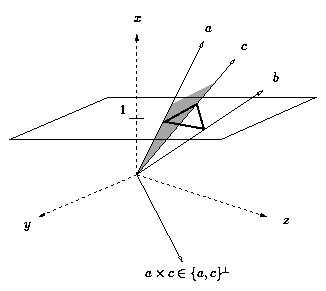
\includegraphics[width=0.7\textwidth]{homogenizedTriangle.jpg}
\caption{Homogenized triangule.}
\label{fig:homogenized-triangle}
\end{figure}


Let $v_1, \dots, v_k$ be the vertices of a polytope $P \subseteq \R^n$, then the \latte v-representation file format is:

\begin{align*}
	k &\: (n+1)\\
	1 &\: v_1\\
	\vdots & \\
	1 &\: v_k
\end{align*}


\example
Note, like \latte h-representations files, a rational-vertex polytope with can be written with integer data by scaling each homogenized vertex. Below are the vertices of a rectangle $(0,0), (2/3,0), (0,1/4), (2/3, 1/4)$:
\begin{verbatim}
4 3
1 0 0
3 2 0
4 0 1
12 8 3
\end{verbatim}

\subsection{\cdd Input Files}
In addition to the formats described above, {\tt LattE} can also
accept input files in standard \cdd format. Below is
an example of \cdd input that is readable into \latte.
\begin{verbatim}
H-representation
begin
4  4  integer
2 -2  4 -1
3 -2 -2  3
6  2 -4 -3
1  2  2  1
end
\end{verbatim}

For a complete description of \cdd file syntax, see the \cdd manual \cite{fukuda}.

\subsection{Non-full dimensional polytopes}

When the input polytope is not full dimensional, \latte projects that polytope such that it becomes full dimensional. This transformation preserves the lattice count and volume of the input polytope. The current \latteInt cannot integrate non-full dimensional polytopes.

\subsection{\latte vs. \cdd file formats}
There are a few key differences between \latte and \cdd file formats.

\begin{enumerate}
	\item \cdd used the file extension *.ine for h-representation files, and *.ext for v-representation files. However, \latte makes no assumption on the file extensions of files. We recommend *.vrep.latte and *.hrep.latte for \latte style files, but you are free to name your files anything.
	\item \cdd also requires ``H-representation'' or ``V-representation'' keywords in the file. Forgetting about the ``linearity'' and ``nonnegative'' keywords, there is no difference between a \latte v- and h-representation file.
%	\item Currently, not all commands work starting from a \cdd v-representation file. --it looks ok now.
\end{enumerate}


\subsection{Polynomials and linear forms}
\label{input-file:polynomial-and-linear-form}

\latteInt can also integrate polynomials and in particular sums of powers of linear forms. Powers of linear forms are the fundamental structure used to integrate. Next, we describe the syntax of polynomials and linear forms

\begin{itemize}
\item A polynomial is represented as a list of its monomials in the form
  \begin{quote}
    \texttt{[{\itshape monomial}$_1$,{\itshape monomial}$_2$,$\dots$]},
  \end{quote}
  where \texttt{{\itshape monomial}$_i$} is represented by
  \begin{quote}
    \texttt{[{\itshape coefficient},[{\itshape exponent-vector}]]}.
  \end{quote}
  For example, $3x_0^2x_1^4x_2^6 + 7x_1^3x_2^5$ is input as \texttt{[[3,[2,4,6]], [7,[0,3,5]]]}. 

\item To deal directly with sums of powers of linear forms, a fundamental data structure in \latteInt, the input format is 
  \begin{quote}
    \texttt{[{\itshape linear-term$_1$}, {\itshape linear-term$_2$}, $\dots$]},
    \end{quote}
    where \texttt{{\itshape linear-term}$_i$} is represented by
    \begin{quote}
      \texttt{[{\itshape coefficient},[{\itshape power},[{\itshape coefficient-vector}]]]}.
    \end{quote}
    For example, $3(2x_0 + 4x_1 + 6x_2)^{10} + 7(3x_1 + 5x_2)^{12}$ is input
    as \texttt{[[3,[10,[2,4,6]]], [7,[12,[0,3,5]]]]}. 


The reason this is useful is because any polynomial can be written as a sum of powers of linear forms, see \cite{howToIntegratePolynomialSimplex}.


\end{itemize}

%*****************************************************************
%*****************************************************************
%*****************************************************************
%*****************************************************************
%*****************************************************************

\section{Running {\tt LattE}}\label{Running LattE}

\subsection{How to use {\tt count}}

{\tt count} has a nice help menu, to view it, run

\begin{verbatim}
	./count --help
\end{verbatim}


The following options control what {\tt count} computes.

\begin{itemize}
\item Count the number of lattice points in polytope $P$, where $P$  is given in a file named ``fileName.hrep.latte'' in different file formats.
	\begin{verbatim}
     ./count fileName.hrep.latte
     ./count --vrep fileName.vrep.latte
     ./count --cdd fileName.ine
	\end{verbatim} 

\item Count the number of lattice points in $nP$, the dilation of $P$ by the integer factor $n$.
	\begin{verbatim}
     ./count --dilation=n fileName.hrep.latte
	\end{verbatim} 
\begin{comment}	
\item Count the number of lattice points in the interior of the  polytope $P$, where $P$ is given in ``fileName''.
	\begin{verbatim}
     ./count --interior fileName.hrep.latte
	\end{verbatim} 
\end{comment}	
\item Use the homogenized Barvinok algorithm \cite{latte3} to count  the number of lattice points in the polytope $P$. Use if number of vertices of $P$ is big compared to the number of constraints. 
	\begin{verbatim}
     ./count --homog fileName.hrep.latte
	\end{verbatim} 
\item Compute the number of lattice points (default)
	\begin{verbatim}
     ./count --count-lattice-points  fileName.hrep.latte
	\end{verbatim} 
\item Compute the multivariate generating function of the set of lattice points of the polyhedron
	\begin{verbatim}
     ./count --multivariate-generating-function  fileName.hrep.latte
	\end{verbatim} 
For unbounded polyhedra, one needs to combine
  this with {\tt --compute-vertex-cones=4ti2}, as other methods in \latte currently refuse to handle unbounded polyhedra. For example, 
	\begin{verbatim}
  	count --compute-vertex-cones=4ti2 --multivariate-generating-function fileName
	\end{verbatim}
  writes the multivariate generating function (in Maple notation) to ``fileName.rat.''
	
	
	
\item Compute the Ehrhart polynomial of an \emph{integral} polytope
	\begin{verbatim}
     ./count --ehrhart-polynomial  fileName.hrep.latte
	\end{verbatim} 
\item Compute the unsimplified Ehrhart series as a univariate rational function
	\begin{verbatim}
     ./count --ehrhart-series  fileName.hrep.latte
	\end{verbatim} 
\item Compute the simplified Ehrhart series as a univariate rational function (needs \maple).
	\begin{verbatim}
     ./count --simplified-ehrhart-series  fileName.hrep.latte
	\end{verbatim} 
\item Compute the first N terms of the Ehrhart series
	\begin{verbatim}
     ./count --ehrhart-taylor=N  fileName.hrep.latte
	\end{verbatim} 
\end{itemize}

The following options relate to the Barvinok algorithm and where introduced by Matthias K\"oppe in \latteMac, see \cite{koeppe:irrational-barvinok}.
\begin{itemize}
\item Triangulate and signed-decompose in the dual space (traditional method, default)
	\begin{verbatim}
     ./count --dual  fileName.hrep.latte
	\end{verbatim} 
\item Triangulate in the dual space, signed-decompose in the primal space using irrationalization
	\begin{verbatim}
     ./count --irrational-primal  fileName.hrep.latte
	\end{verbatim} 
\item Triangulate and signed-decompose in the primal space  using irrationalization
	\begin{verbatim}
     ./count --irrational-all-primal  fileName.hrep.latte
	\end{verbatim} 
	This gives a new method for computing Ehrhart polynomials of integral polytopes 
   in the primal space
	\begin{verbatim}
     ./count --all-primal --ehrhart-polynomial fileName.hrep.latte
	\end{verbatim} 
   
\item  Decompose cones down to an index (determinant) of N instead down to unimodular cones (which have an index of 1).
	\begin{verbatim}
     ./count --maxdet=N  fileName.hrep.latte
	\end{verbatim} 
\item Do not signed-decompose simplicial cones
	\begin{verbatim}
     ./count --no-decomposition   fileName.hrep.latte
	\end{verbatim} 
\item Use polynomial substitution for specialization (traditional method, default)
	\begin{verbatim}
     ./count --polynomial  fileName.hrep.latte
	\end{verbatim} 	
\item Use exponential substitution for specialization (recommended for maxdet larger than 1)
	\begin{verbatim}
     ./count --exponential   fileName.hrep.latte
	\end{verbatim} 	
			
\end{itemize}


\textbf{REMARK}  The functionality of the \latte v1.2 {\tt ehrhart} command has been merged into {\tt count}:

\begin{verbatim} 
	count --ehrhart-series FILENAME
	
	      (replaces: ehrhart FILENAME)

	count --simplified-ehrhart-series FILENAME

	      (replaces: ehrhart simplify FILENAME)

	count --ehrhart-taylor=N FILENAME

	      (replaces: ehrhart N FILENAME)
\end{verbatim}

The {\tt ehrhart} program is still available, but it does not accept
   the new command-line options of {\tt count}.

\subsection{How to use {\tt integrate}}

Like {\tt count}, {\tt integrate} has a help menu. To view the menu, run

\begin{verbatim}
	./integrate --help
\end{verbatim}	

There are two different integration (and volume) algorithms. The triangulation method triangulates the entire polytope and integrates over each simplex. In the cone decomposition method we integrate over each cone, possibly triangulating it first. Unlike other integration software, \latte integrates polynomials and powers of linear forms in exact arithmetic.

\begin{itemize}
\item Integrates using the cone-decomposition method.
	\begin{verbatim}
     --cone-decompose
	\end{verbatim} 	
\item Integrates using the triangulation method.
	\begin{verbatim}
     --triangulate
	\end{verbatim} 	
\item Sets what you want to compute: a volume or an integral.
	\begin{verbatim}
     --valuation=integrate
     --valuation=volume
	\end{verbatim} 	
\item Prints the cone-decomposition rational function for volumes
	\begin{verbatim}
     --valuation=volume --cone-decompose --print-cone-decompose-function
	\end{verbatim} 	
\item Sets the file that contains the polynomial or powers of linear forms. If this option is not set, and the valuation is integration, the polynomial or powers of linear forms will be read from stdin.
	\begin{verbatim}
     --monomials=FILE
     --linear-forms=FILE
	\end{verbatim} 	
\end{itemize}

\example
Let us view a few examples of the above options

\begin{itemize}
\item Integrates a polynomial in file ``FILE'' using the triangulation method. 
	\begin{verbatim}
	./integrate --valuation=integral --triangulate --monomials=FILE fileName.hrep.latte
	\end{verbatim} 	
\item Find a volume using the cone decomposition method from a \latte v-representation file.
	\begin{verbatim}
	./integrate --valuation=volume --cone-decompose --vrep fileName.vrep.latte
	\end{verbatim} 	
\item If an integration method is not given, \latteInt computes the integral with \emph{both} methods. This cal also be done by the {\tt --all} option. The next two commands do the same thing: find a volume using both methods from a \latte v-representation file.
	\begin{verbatim}
	./integrate --valuation=volume --vrep fileName.vrep.latte
	./integrate --valuation=volume --all --vrep fileName.vrep.latte	
	\end{verbatim} 	
\end{itemize}
           

\subsection{Options common to both {\tt count} and {\tt integrate}}

A common subproblem in counting lattice points and integration requires finding triangulations and tangent cones. Also, there are many different software tools available to do this. Instead of reinventing the wheel, \latte links with other software tools to compute these basic objects. In this section, we describe how you can control which software tool is used.

\begin{itemize}
\item The \fourtitwo program can be used instead of {\tt cddlib} and {\tt CDD+}
  to compute the vertex cones of polytopes, triangulations, and duals of cones.
  In many cases, \fourtitwo is faster.
  
  \begin{verbatim}
	--compute-vertex-cones={cdd,4ti2}
	--triangulation={cddlib,4ti2}
	--dualization={cdd,4ti2}
  \end{verbatim}

\item By default, \latte assumes the h-representation may contain redundant hyperplanes and tries to find and remove them. You can control how much more \latte should spend checking the input h-representation with the following option.

	\begin{verbatim}
	--redundancy-check={none,cddlib,full-cddlib}.
	\end{verbatim}

	\begin{itemize}
  	\item ``full-cddlib'' (the default) uses cddlib to compute an irredundant
    system of linear equations and inequalities describing the
    polyhedron.  This corresponds to the traditional \latte behavior;
    it can be expensive.

	\item ``cddlib'' (used to be the default in the 1.2+mk-0.9.x series) uses
    cddlib to compute some implicit linearities only; it often fails
    but is faster than full-cddlib.

	\item ``none'' does nothing, the input description of the polytope should
    be irredundant.
		
	\end{itemize}

\end{itemize}


\subsection{Optimization}


\latte can also optimize over the integer points of a polytope. However, this part of the software is not as stable as the rest of the code. The optimization executables {\bf require} a cost vector specified in ``fileName.cost'' if the polytope file is named ``fileName.''

\begin{itemize}
\item Maximizes/Minimizes a given linear cost function over the lattice
  points in the polytope. The Digging algorithm
  \cite{latte3} is used. Optimal point and optimal value is returned. 
\begin{verbatim}
     ./latte-maximize fileName
     ./latte-minimize fileName
\end{verbatim} 
\item Maximizes/Minimizes a given linear cost function over the lattice
  points in the polytope. The Binary search
  algorithm is used. Only optimal value is returned. 
\begin{verbatim}
     ./latte-maximize bbs fileName
     ./latte-minimize bbs fileName
\end{verbatim} 
\end{itemize}



%\newpage

\section{Downloading and Installing {\tt LattE}}

{\tt LattE} is downloadable from the following website:

\makebox[12 cm]{http://www.math.ucdavis.edu/$\sim$latte/}



\latte uses the GNU Autoconf and Automake tools. Please see the {\tt README} file in the \latte directory for detailed directions for installing \latte.

\begin{comment}
\textbf{Step 1: Create directory for {\tt LattE}}

\begin{verbatim}
     mkdir latte
\end{verbatim}

\textbf{Step 2: Download ``latte\_v1.1.tar.gz'' to directory ``latte''}

\begin{verbatim}
     Download ``latte_v1.1.tar.gz'' from
\end{verbatim}

\makebox[12 cm]{http://www.math.ucdavis.edu/$\sim$latte/downloads/}
 
(If you have never downloaded a file from the internet: A click with
your right mouse button onto the file name on the webpage should do
the trick. In any case, if you do not succeed, ask your system
administrator, a friend, or send us an email.) 

\textbf{Step 3: Change to directory for ``latte''}

\begin{verbatim}
     cd latte
\end{verbatim}

\textbf{Step 4: Unzip and untar the archive} 

\begin{verbatim}
     gunzip latte_v1.1.tar.gz
     tar xvf latte_v1.1.tar
\end{verbatim}

\textbf{Step 5: Make ``install'' executable} 

\begin{verbatim}
     chmod 700 install
\end{verbatim}

\textbf{Step 6: Install {\tt LattE}} 

\begin{verbatim}
     ./install
\end{verbatim}

\end{comment}






%\newpage

\section{A Brief Tutorial}
In this section we invite the reader to follow along a few examples
that show how to use {\tt LattE} and also how to counter-check
results.

\subsection{Counting Magic Squares}
Our first example deals with counting magic $4\times 4$ squares. We 
call a $4\times 4$ array of nonnegative numbers a magic square if the
sums of the $4$ entries along each row, along each column and along
the two main diagonals equals the same number $s$, the magic
constant. Let us start with counting magic $4\times 4$ squares that
have the magic constant $1$. Associating variables $x_1,\ldots,x_{16}$ with
the $16$ entries, the conditions of a magic $4\times 4$ square of
magic sum $1$ can be encoded into the following input file
``EXAMPLES/magic4x4'' for {\tt LattE}.
\begin{verbatim}
10 17
1 -1 -1 -1 -1  0  0  0  0  0  0  0  0  0  0  0  0
1  0  0  0  0 -1 -1 -1 -1  0  0  0  0  0  0  0  0
1  0  0  0  0  0  0  0  0 -1 -1 -1 -1  0  0  0  0
1  0  0  0  0  0  0  0  0  0  0  0  0 -1 -1 -1 -1
1 -1  0  0  0 -1  0  0  0 -1  0  0  0 -1  0  0  0
1  0 -1  0  0  0 -1  0  0  0 -1  0  0  0 -1  0  0
1  0  0 -1  0  0  0 -1  0  0  0 -1  0  0  0 -1  0
1  0  0  0 -1  0  0  0 -1  0  0  0 -1  0  0  0 -1
1 -1  0  0  0  0 -1  0  0  0  0 -1  0  0  0  0 -1
1  0  0  0 -1  0  0 -1  0  0 -1  0  0 -1  0  0  0
linearity 10 1 2 3 4 5 6 7 8 9 10
nonnegative 16 1 2 3 4 5 6 7 8 9 10 11 12 13 14 15 16
\end{verbatim}
Now we simply invoke the counting function of {\tt LattE} by typing:
\begin{verbatim}
    ./count EXAMPLES/magic4x4
\end{verbatim}

The last couple of lines that {\tt LattE} prints to the screen
look as follows:
\begin{verbatim}
Total Unimodular Cones: 418
Maximum number of simplicial cones in memory at once: 27

*****  Total number of lattice points: 8  ****

Computation done.
Time: 1.24219 sec
\end{verbatim}
Therefore, there are exactly $8$ magic $4\times 4$ squares that
have the magic constant $1$. This is not yet impressive, as we could
have done that by hand. Therefore, let us try and find the
corresponding number for the magic constant $12$. Since this problem
is a dilation (by factor $12$) of the original problem, we do not have
to create a new file. Instead, we use the option ``dilation'' to indicate
that we want to count the number of lattice points of a dilation of
the given polytope:
\begin{verbatim}
    ./count --dilation=12 EXAMPLES/magic4x4
\end{verbatim}
The last couple of lines that {\tt LattE} prints to the screen
look as follows:
\begin{verbatim}
Total Unimodular Cones: 418
Maximum number of simplicial cones in memory at once: 27

*****  Total number of lattice points: 225351  ****

Computation done.
Time: 1.22656 sec
\end{verbatim}
Therefore, there are exactly $225351$ magic $4\times 4$ squares that
have the magic constant $12$. (We would NOT want to do THAT one by
hand, would we?!) 

Here is some amazing observation: the running time of {\tt LattE}
is roughly the same for counting magic squares of sum $1$ and of sum
$12$. This phenomenon is due to the fact that the main part of the
computation, the creation of the generating function that encodes all
lattice points in the polytope, is nearly identical in both cases.

Although we may be already happy with these simple counting results,
let us be a bit more ambitious and and let us find a counting formula
that, for given magic sum $s$, returns the number of magic 
$4\times 4$ squares that have the magic constant $s$.

For this, simply type (note that {\tt LattE} invokes {\tt Maple} to
simplify intermediate expressions):
\begin{verbatim}
    ./count --simplified-ehrhart-series EXAMPLES/magic4x4
\end{verbatim}
The last couple of lines that {\tt LattE} prints to the screen looks
as follows:
\begin{verbatim}
Rational function written to EXAMPLES/magic4x4.rat

Computation done. 
Time: 0.724609 sec
\end{verbatim}
We are informed that this call created a file ``EXAMPLES/magic4x4.rat''
containing the Ehrhart series as a rational function:
{\small
\begin{verbatim}
(t^8+4*t^7+18*t^6+36*t^5+50*t^4+36*t^3+18*t^2+4*t+1)/(-1+t)^4/(-1+t^2)^4
\end{verbatim}
}
Now we could use {\tt Maple} (or your favorite computer algebra
software) to find a series expansion of this expression. 
\begin{eqnarray*}
& & 
\frac{t^8+4*t^7+18*t^6+36*t^5+50*t^4+36*t^3+18*t^2+4*t+1}{(-1+t)^4(-1+t^2)^4}\\
& = & 1+8t^1+48t^2+200t^3+675t^4+1904t^5+4736t^6+10608t^7+21925t^8+\\
& & 42328t^9+77328t^{10}+134680t^{11}+225351t^{12}+364000t^{13}+570368t^{14}+\\
& & 869856t^{15}+{O}(t^{16})\\
\end{eqnarray*}
The summands $8t$ and $225351t^{12}$ reconfirm our previous
counts.

Although this rational function encodes the full Ehrhart series, it is
not always as easy to compute as for magic $4\times 4$ squares. As it
turns out, adding and simplifying rational functions, although in just
one variable $t$, can be extremely costly due to the high powers in
$t$ and due to long integer coefficients that appear.

However, even if we cannot compute the full Ehrhart series, we can at
least try and find the first couple of terms of it. 
\begin{verbatim}
    ./count --ehrhart-taylor=15 EXAMPLES/magic4x4
\end{verbatim}
The last couple of lines that {\tt LattE} prints to the screen
look as follows:
\begin{verbatim}
Memory Save Mode: Taylor Expansion:
1
8t^1
48t^2
200t^3
675t^4
1904t^5
4736t^6
10608t^7
21925t^8
42328t^9
77328t^10
134680t^11
225351t^12
364000t^13
570368t^14
869856t^15
Computation done.
Time: 1.83789 sec
\end{verbatim}
Again, our previous counts are reconfirmed.

Nice, but the more terms we want to compute the more time-consuming
this task becomes. Clearly, if we could find sufficiently many
terms, we could compute the full Ehrhart series expansion in terms of
a rational function by interpolation.

\subsection{Counting Lattice Points in the $24$-Cell}
Our next example deals with a well-known combinatorial object, the
$24$-cell. Its description is given in the file ``EXAMPLES/24\_cell'':
\begin{verbatim}
24 5 
2 -1  1 -1 -1
1  0  0 -1  0
2 -1  1 -1  1
2 -1  1  1  1
1  0  0  0  1
1  0  1  0  0
2  1 -1  1 -1
2  1  1 -1  1
2  1  1  1  1
1  1  0  0  0
2  1  1  1 -1
2  1  1 -1 -1
2  1 -1  1  1
2  1 -1 -1  1
2  1 -1 -1 -1
1  0  0  1  0
2 -1  1  1 -1
1  0  0  0 -1
2 -1 -1  1 -1
1  0 -1  0  0
2 -1 -1  1  1
2 -1 -1 -1  1
2 -1 -1 -1 -1
1 -1  0  0  0
\end{verbatim}
Now we invoke the counting function of {\tt LattE} by typing:
\begin{verbatim}
    ./count EXAMPLES/24_cell
\end{verbatim}
The last couple of lines that {\tt LattE} prints to the screen
look as follows:
\begin{verbatim}
Total Unimodular Cones: 240
Maximum number of simplicial cones in memory at once: 30

*****  Total number of lattice points: 33  ****

Computation done. 
Time: 0.429686 sec
\end{verbatim}
Therefore, there are exactly $33$ lattice points in the $24$-cell. We
get the same result by using the homogenized Barvinok algorithm:
\begin{verbatim}
    ./count --homog EXAMPLES/24_cell
\end{verbatim}
The last couple of lines that {\tt LattE} prints to the screen
look as follows:
\begin{verbatim}
Memory Save Mode: Taylor Expansion:

****  Total number of lattice points is: 33  ****

Computation done. 
Time: 0.957031 sec
\end{verbatim}

\begin{comment}
But how many of these $33$ points lie in the interior of the
$24$-cell?
\begin{verbatim}
    ./count --interior EXAMPLES/24_cell
\end{verbatim}
The last couple of lines that {\tt LattE} prints to the screen
look as follows:
\begin{verbatim}
Reading .ext file...


*****  Total number of lattice points: 1 ****
\end{verbatim}
Therefore, there only one of the $33$ lattice points in the $24$-cell
lies in the interior.
\end{comment}




\subsection{Integrating over a polytope}

Let us integrate the polynomial $w^2x^2y^4z^8 -3/8x^2$ and the power of a linear form $3(w +2x + 4y + 6z)^{10}$ over the $24$-cell.

 

Create a file named ``even.polynomial'' that has on its first line the polynomial. See Section \ref{input-file:polynomial-and-linear-form} for a review of the syntax.
	
	\begin{verbatim}
	[[1,[2,2,4,8]], [-3/8,[0,2,0,0]]]
	\end{verbatim}

After running the integration command using the triangulation method
	\begin{verbatim}
	./integrate --valuation=integrate --triangulate --monomials=even.polynomial 24_cell
	\end{verbatim}


we see that the two monomials where decomposed into 406 powers of linear forms and the answer is


\begin{verbatim}
starting to integrate 406 linear forms.

Integration (using the triangulation method)
     Answer: -110535307/170059500
     Decimal: -0.64998019516698567266162725399052
     Time: 1.92 sec
Computational time (algorithms + processing + program control)
     Total time: 2.00 sec
\end{verbatim}



Now create a new file named ``power10.linearforms'' that has in its first line the power of a linear form:

	\begin{verbatim}
	[[3,[10,[1,2,4,6]]]]
	\end{verbatim}
	
Then integrate this power of a linear form over the 24\_cell using the cone decomposition method with the following command:	
	\begin{verbatim}
	./integrate --cone-decompose --linear-forms=power10.linearforms  24_cell
	\end{verbatim}
	
We see the answer is computed very quickly.
	
\begin{verbatim}	
Integration (using the cone decomposition method)
     Answer: 59555515086/77
     Decimal: 773448247.87012987012987012987013
     Time: 0.02 sec
Computational time (algorithms + processing + program control)
     Total time: 0.07 sec
\end{verbatim}	
	
\begin{figure}[thb]
	\centering
	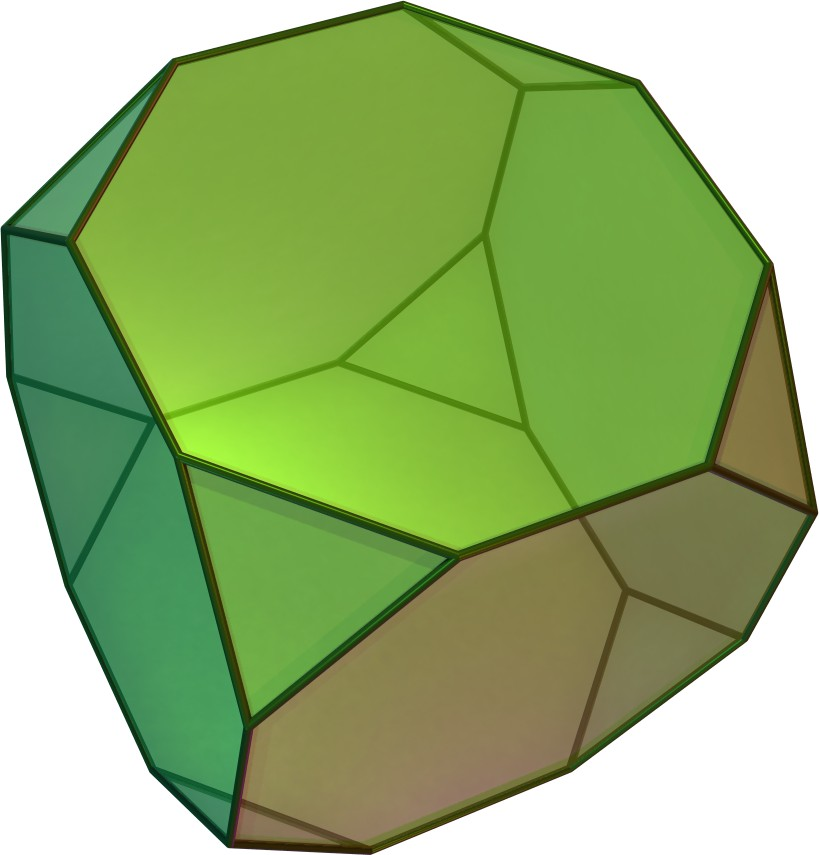
\includegraphics[width=0.3\textwidth]{truncatedCube.jpg}
\caption{The truncated cube.}
	\label{fig:truncated-cube}
\end{figure}	
	
For the next example, consider the truncated cube in Figure \ref{fig:truncated-cube}	

	
The vertices are
\begin{verbatim}
24 4
1 3 1 1
1 3 1 -1
1 3 -1 1
1 3 -1 -1
1 -3 1 1
1 -3 1 -1
1 -3 -1 1
1 -3 -1 -1
1 1 3 1
1 1 3 -1
1 1 -3 1
1 1 -3 -1
1 -1 3 1
1 -1 3 -1
1 -1 -3 1
1 -1 -3 -1
1 1 1 3
1 1 1 -3
1 1 -1 3
1 1 -1 -3
1 -1 1 3
1 -1 1 -3
1 -1 -1 3
1 -1 -1 -3
\end{verbatim}

This time, let us enter the polynomial $x^{40}y^{40}z^{40}$ from stdin, which
will be decomposed into $68,920$ powers of linear forms. Run
	
	\begin{verbatim}
	./integrate --cone-decompose --triangulation=4ti2 --vrep truncatedCube.vrep.latte 
	\end{verbatim}

and type
	\begin{verbatim}
	p [[1,[40,40,40]]]
	\end{verbatim}


We see the exact answer is 
\begin{displaymath}
\frac{93991283632941965714919247928639002510318209692293688827363993265109276641003769553256}{2795239135836124463932439643671211584534957465679791608181565}
\end{displaymath}
	
This answer displays the power of using exact rational arithmetic!	


\subsection{Example of Optimization with \latte}

Next, let us solve the problem ``cuww1'' \cite{cuww,latte3}. Its
description is given in the file ``EXAMPLES/cuww1'': 
\begin{verbatim}
1 6
89643482 -12223 -12224 -36674 -61119 -85569
linearity 1 1
nonnegative 5 1 2 3 4 5
\end{verbatim}
The cost function can be found in the file ``EXAMPLES/cuww1.cost'':
\begin{verbatim}
1 5
213 -1928 -11111 -2345 9123 
\end{verbatim}
Now let us maximize this cost function over the given knapsack
polytope. Note that by default, the digging algorithm as described in
\cite{latte3} is used.
\begin{verbatim}
    ./latte-maximize EXAMPLES/cuww1
\end{verbatim}
The last couple of lines that {\tt LattE} prints to the screen
look as follows:
{\small
\begin{verbatim}
Finished computing a rational function. 
Time: 0.158203 sec.

There is one optimal solution. 		

No digging.
An optimal solution for [213 -1928 -11111 -2345 9123] is: [7334 0 0 0 0].
The projected down opt value is: 191928257104
The optimal value is: 1562142.
The gap is: 7995261.806
Computation done.
Time: 0.203124 sec.
\end{verbatim}
}
The solution $(7334,0,0,0,0)$ is quickly found. Now let us try to
find the optimal value again by a different algorithm, the binary
search algorithm.
\begin{verbatim}
    ./latte-maximize bbs EXAMPLES/cuww1
\end{verbatim}
The last couple of lines that {\tt LattE} prints to the screen
look as follows:
\begin{verbatim}
Total of Iterations: 26
The total number of unimodular cones: 125562
The optimal value: 1562142

The number of optimal solutions: 1
Time: 0.042968
\end{verbatim}
Note that we get the same optimal value, but no optimal solution is
provided.	
\section{Release Information}

\subsection{System Requirements}

\subsubsection{Platform} 
The binaries for \latte v1.1 as well as for {\tt cdd} (by
K. Fukuda \cite{fukuda}) are for platforms that run Unix, that is, Mac and Linux.

\subsubsection{Memory Requirements} 
The memory requirements are essentially problem dependent; however,
{\tt LattE count} runs in a ``memory saving mode'' whenever appropriate.
In this mode {\tt count} rarely uses more than around 20 MB beyond the
amount of memory needed to calculate triangulations. 

\subsection{Additional \maple Connection}
The call
\begin{verbatim}
./count --simplified-ehrhart-series  fileName
\end{verbatim}
requires \maple for simplifications of expressions. It should be
sufficient to have a copy of \maple installed on your machine,
without any additional special configuration required.  \latte
will still run even if \maple is not installed, but this
simplification feature to ``count'' will not be available. 

We have tested this connection with \maple 5.1, 8.0, and 14.0 and experienced
no problem. Please let us know about any problem you experience with
our connection to \maple.

\subsection{File Descriptions} 
\label{section:file-descriptions}
The {\tt LattE} Linux release consists a single archive file,
\textbf{latte\_v1.*.tar.gz}. The archive contains the following files:

\begin{tabular}{|l|l|}
\hline
Name & Description\\
\hline 
%\hline
& \\
count & Main program executables\\
ehrhart & \\
latte-maximize & \\
latte-minimize & \\
integrate      & \\
& \\

simplify2.add & additional files used by {\tt LattE}\\
redcheck & ($\leftarrow$ modified from {\tt cdd} library) \\
install & \\
& \\
cdd & external {\tt cdd} software executable used by {\tt LattE},\\
& original name in {\tt cdd}: cddr+\_gmp\\
& \\
\hline
& \\
EXAMPLES/ & Subdirectory containing sample input files\\
& \\
\hline
& \\
manual.pdf & User's guide \\
%manual.pdf & \\
& \\
\hline 
& \\
code/ & {\tt LattE} source code (including {\tt NTL}, {\tt cdd} and {\tt cdd lib})\\
& \\
\hline 
& \\
gpl.txt & GNU General Public License agreement\\
& \\
\hline 
\end{tabular}

\subsection{License Agreement}

This program is free software; you can redistribute it and/or
modify it under the terms of the version 2 of GNU General Public
License as published by the Free Software Foundation.

This program is distributed in the hope that it will be useful,
but WITHOUT ANY WARRANTY; without even the implied warranty of
MERCHANTABILITY or FITNESS FOR A PARTICULAR PURPOSE. See the GNU
General Public License for more details. (The careful user can find
an install script for the source code in the directory ``code/''.)

You should have received a copy of the GNU General Public License
along with this program; see the file COPYING. If not, write to
the Free Software Foundation, Inc., 59 Temple Place - Suite 330,
Boston, MA 02111-1307, USA.

We have included a copy of the GNU General Public License also at the
end of this document.

\subsection{How to Cite {\tt LattE}}

Although {\tt LattE} is free software, your acknowledgment
is requested.  If {\tt LattE} is useful in your research or
applications please acknowledge it by referencing this manual as

De Loera, J.A., Dutra, B., K\"oppe, M., Moreinis, S.,
Pinto, G., Wu, J.\\ 
{\em A User's Guide for {\tt LattE integrale} \latteV}, 2011, 
software package \latte is available at 
{\tt http://www.math.ucdavis.edu/$\sim$latte/}
	
\subsection{The {\tt LattE} Team}
\begin{description}
\item[Project directors]  Prof. Jes\'us A. De Loera and Prof. Matthias K\"oppe
\item[Students currently working on the project] Brandon Dutra
\item[Distinguished \latte Scientists, Collaborators and Advisors] \hfill \\
	\begin{itemize} 
		\item Dr. Raymond Hemmecke (\latte v1.2)
		\item Prof. Ruriko Yoshida (\latte v1.2)
		\item Dr. David Haws (\latte v1.2)
		\item Dr. Peter Huggins (\latte v1.2)
		\item Prof. Tyrrell McAllister
		\item Prof. Velleda Baldoni
		\item Prof. Nicole Berline
		\item Prof. Michele Vergne
		\item Prof. Alexander Barvinok
		\item Prof. Bernd Sturmfels 
	\end{itemize}
\item[Alumni of the project]	\hfill \\
	\begin{itemize}
		\item Gregory Pinto	(\latteInt)
		\item Stanislav Moreinis (\latteInt)
		\item Jianqiu Wu (\latteInt)
		\item Jeremy Tauzer (\latte v1.2)
		\item Jonathan Brooks (\latte v1.2)
		\item Carol Shih (\latte v1.2)
		\item Esteban Pauli (\latte v1.2)
		\item Mike Zhang	(\latte v1.2)
	\end{itemize}
\end{description}

\subsection{Acknowledgments}

\par {\tt LattE} currently uses many wonderful pieces of software.
First is {\tt cdd} \cite{fukuda}, developed by Komei Fukuda, whose webpage can be
found at:

\makebox[12 cm]{http://www.cs.mcgill.ca/$\sim$fukuda/}

Next, \latte uses \fourtitwo \cite{4ti2} whose webpage can be found at:

\makebox[12 cm]{http://www.4ti2.de}

{\tt cdd} and \fourtitwo is used for finding vertices of polytopes and the
triangulation of cones.

In addition, {\tt LattE} currently uses NTL, a
Library for doing Number Theory, written by Victor Shoup \cite{shoup},
for LLL algorithm, matrix manipulations, storing variable length
integers, and floating point numbers.  NTL can be found at:

\makebox[12cm]{http://shoup.net/ntl/}

We are truly grateful to Velleda Baldoni, Alexander Barvinok, Nicole Berline, Komei Fukuda, Tyrrell McAllister, Dmitrii Pasechnik, Michele Vergne, and Bernd Sturmfels for several suggestions and
useful conversations that improved our software.  We thank the National
Science Foundation for support to this project via NSF grants DMS-0309694, 
DMS-0073815, DMS-0914107 and DMS-0914873. Most of the students were supported by those
grants and by summer fellowships provided through the UC Davis VIGRE grants
DMS-0135345 and DMS-0636297.


%\newpage

\bibliographystyle{amsabbrv}
\bibliography{bibliography}

\begin{comment}
\begin{thebibliography}{99}
\bibitem{4ti2}{4ti2 team}{\em \: 4ti2---A software package for algebraic, geometric and 
combinatorial problems on linear spaces}. Available at \url{www.4ti2.de}.
\bibitem{howToIntegratePolynomialSimplex} {V. Baldoni, N. Berline, J. A. De 
Loera, M. K{\"o}ppe, and M. Vergne} {\em How to integrate a polynomial over a
simplex}, Mathematics of Computation 80 (2011), no. 273, 297–325.
\bibitem{BarviPom} {Barvinok, A.I. and Pommersheim, J.} {\em An
algorithmic theory of lattice points in polyhedra}, in: {\sl New
Perspectives in Algebraic Combinatorics} (Berkeley, CA, 1996-1997),
91-147, Math. Sci. Res.  Inst. Publ. 38, Cambridge Univ. Press,
Cambridge, 1999.
\bibitem{cuww}{Cornu\'ejols, G., Urbaniak, R., Weismantel, R., Wolsey, L.A.} 
{\em Decomposition of integer programs and of generating sets.}  
R. E. Burkard, G. J. Woeginger, eds., {\em Algorithms}--ESA 97. 
Lecture Notes in Computer Science 1284, Springer-Verlag, 92--103, 1997. 
\bibitem{latte1}{De Loera, J.A., Hemmecke, R., Tauzer, J., and Yoshida, R.}
{\em Effective lattice point counting in rational convex polytopes},
Journal of Symbolic Computation, Volume 38, Issue 4, Symbolic Computation in Algebra and Geometry, October 2004, Pages 1273-1302, ISSN 0747-7171, DOI: 10.1016/j.jsc.2003.04.003.
\bibitem{latte2}{De Loera, J.A., Haws, D., Hemmecke, R., Huggins, P.,
Sturmfels, B., and Yoshida, R.} {\em Short rational functions for
toric algebra and applications}, e-print, Available via 
\url{http://front.math.ucdavis.edu/math.CO/0307350}, 2003.
\bibitem{latte3}{De Loera, J.A., Haws, D., Hemmecke, R., Huggins, P.,
and Yoshida, R.} {\em Three kinds of integer programming algorithms based on
  {B}arvinok's rational functions}, manuscript, 2003.
\bibitem{fukuda} {Fukuda, K.} {\tt cdd} and {\tt cdd+}, {\em The {\tt cdd}
and {\tt cdd} plus}, available via
\url{http://www.cs.mcgill.ca/~fukuda/soft/cdd_home/cdd.html}.
\bibitem{shoup} {Shoup, V.} {\em {\tt NTL}, A library for doing Number
Theory}, available via \url{http://shoup.net/ntl/}. 
\bibitem{sturmfels} {Sturmfels, B.} {\em Gr\"obner bases and convex
polytopes}, university lecture series, vol. 8, AMS, Providence RI,
1996.
\bibitem{stanley}{Stanley, R.P.} {\em Enumerative Combinatorics}, 
Volume I, Cambridge, 1997.
\end{thebibliography}	

\end{comment}

%\newpage



%****************************************************************************
%****************************************************************************
%****************************************************************************
%****************************************************************************
%****************************************************************************
%****************************************************************************
%****************************************************************************
%****************************************************************************
%****************************************************************************
%****************************************************************************
%****************************************************************************
%****************************************************************************
\section{The GNU General Public License}


\begin{center}
{\parindent 0in

Version 2, June 1991

Copyright \copyright\ 1989, 1991 Free Software Foundation, Inc.

\bigskip

59 Temple Place - Suite 330, Boston, MA  02111-1307, USA

\bigskip

Everyone is permitted to copy and distribute verbatim copies
of this license document, but changing it is not allowed.
}
\end{center}

\begin{center}
{\bf\large Preamble}
\end{center}


The licenses for most software are designed to take away your freedom to
share and change it.  By contrast, the GNU General Public License is
intended to guarantee your freedom to share and change free software---to
make sure the software is free for all its users.  This General Public
License applies to most of the Free Software Foundation's software and to
any other program whose authors commit to using it.  (Some other Free
Software Foundation software is covered by the GNU Library General Public
License instead.)  You can apply it to your programs, too.

When we speak of free software, we are referring to freedom, not price.
Our General Public Licenses are designed to make sure that you have the
freedom to distribute copies of free software (and charge for this service
if you wish), that you receive source code or can get it if you want it,
that you can change the software or use pieces of it in new free programs;
and that you know you can do these things.

To protect your rights, we need to make restrictions that forbid anyone to
deny you these rights or to ask you to surrender the rights.  These
restrictions translate to certain responsibilities for you if you
distribute copies of the software, or if you modify it.

For example, if you distribute copies of such a program, whether gratis or
for a fee, you must give the recipients all the rights that you have.  You
must make sure that they, too, receive or can get the source code.  And
you must show them these terms so they know their rights.

We protect your rights with two steps: (1) copyright the software, and (2)
offer you this license which gives you legal permission to copy,
distribute and/or modify the software.

Also, for each author's protection and ours, we want to make certain that
everyone understands that there is no warranty for this free software.  If
the software is modified by someone else and passed on, we want its
recipients to know that what they have is not the original, so that any
problems introduced by others will not reflect on the original authors'
reputations.

Finally, any free program is threatened constantly by software patents.
We wish to avoid the danger that redistributors of a free program will
individually obtain patent licenses, in effect making the program
proprietary.  To prevent this, we have made it clear that any patent must
be licensed for everyone's free use or not licensed at all.

The precise terms and conditions for copying, distribution and
modification follow.

\begin{center}
{\Large \sc Terms and Conditions For Copying, Distribution and
  Modification}
\end{center}


%\renewcommand{\theenumi}{\alpha{enumi}}
\begin{enumerate}

\addtocounter{enumi}{-1}

\item 

This License applies to any program or other work which contains a notice
placed by the copyright holder saying it may be distributed under the
terms of this General Public License.  The ``Program'', below, refers to
any such program or work, and a ``work based on the Program'' means either
the Program or any derivative work under copyright law: that is to say, a
work containing the Program or a portion of it, either verbatim or with
modifications and/or translated into another language.  (Hereinafter,
translation is included without limitation in the term ``modification''.)
Each licensee is addressed as ``you''.

Activities other than copying, distribution and modification are not
covered by this License; they are outside its scope.  The act of
running the Program is not restricted, and the output from the Program
is covered only if its contents constitute a work based on the
Program (independent of having been made by running the Program).
Whether that is true depends on what the Program does.

\item You may copy and distribute verbatim copies of the Program's source
  code as you receive it, in any medium, provided that you conspicuously
  and appropriately publish on each copy an appropriate copyright notice
  and disclaimer of warranty; keep intact all the notices that refer to
  this License and to the absence of any warranty; and give any other
  recipients of the Program a copy of this License along with the Program.

You may charge a fee for the physical act of transferring a copy, and you
may at your option offer warranty protection in exchange for a fee.

\item

You may modify your copy or copies of the Program or any portion
of it, thus forming a work based on the Program, and copy and
distribute such modifications or work under the terms of Section 1
above, provided that you also meet all of these conditions:

\begin{enumerate}

\item 

You must cause the modified files to carry prominent notices stating that
you changed the files and the date of any change.

\item

You must cause any work that you distribute or publish, that in
whole or in part contains or is derived from the Program or any
part thereof, to be licensed as a whole at no charge to all third
parties under the terms of this License.

\item
If the modified program normally reads commands interactively
when run, you must cause it, when started running for such
interactive use in the most ordinary way, to print or display an
announcement including an appropriate copyright notice and a
notice that there is no warranty (or else, saying that you provide
a warranty) and that users may redistribute the program under
these conditions, and telling the user how to view a copy of this
License.  (Exception: if the Program itself is interactive but
does not normally print such an announcement, your work based on
the Program is not required to print an announcement.)

\end{enumerate}


These requirements apply to the modified work as a whole.  If
identifiable sections of that work are not derived from the Program,
and can be reasonably considered independent and separate works in
themselves, then this License, and its terms, do not apply to those
sections when you distribute them as separate works.  But when you
distribute the same sections as part of a whole which is a work based
on the Program, the distribution of the whole must be on the terms of
this License, whose permissions for other licensees extend to the
entire whole, and thus to each and every part regardless of who wrote it.

Thus, it is not the intent of this section to claim rights or contest
your rights to work written entirely by you; rather, the intent is to
exercise the right to control the distribution of derivative or
collective works based on the Program.

In addition, mere aggregation of another work not based on the Program
with the Program (or with a work based on the Program) on a volume of
a storage or distribution medium does not bring the other work under
the scope of this License.

\item
You may copy and distribute the Program (or a work based on it,
under Section 2) in object code or executable form under the terms of
Sections 1 and 2 above provided that you also do one of the following:

\begin{enumerate}

\item

Accompany it with the complete corresponding machine-readable
source code, which must be distributed under the terms of Sections
1 and 2 above on a medium customarily used for software interchange; or,

\item

Accompany it with a written offer, valid for at least three
years, to give any third party, for a charge no more than your
cost of physically performing source distribution, a complete
machine-readable copy of the corresponding source code, to be
distributed under the terms of Sections 1 and 2 above on a medium
customarily used for software interchange; or,

\item

Accompany it with the information you received as to the offer
to distribute corresponding source code.  (This alternative is
allowed only for noncommercial distribution and only if you
received the program in object code or executable form with such
an offer, in accord with Subsection b above.)

\end{enumerate}


The source code for a work means the preferred form of the work for
making modifications to it.  For an executable work, complete source
code means all the source code for all modules it contains, plus any
associated interface definition files, plus the scripts used to
control compilation and installation of the executable.  However, as a
special exception, the source code distributed need not include
anything that is normally distributed (in either source or binary
form) with the major components (compiler, kernel, and so on) of the
operating system on which the executable runs, unless that component
itself accompanies the executable.

If distribution of executable or object code is made by offering
access to copy from a designated place, then offering equivalent
access to copy the source code from the same place counts as
distribution of the source code, even though third parties are not
compelled to copy the source along with the object code.

\item
You may not copy, modify, sublicense, or distribute the Program
except as expressly provided under this License.  Any attempt
otherwise to copy, modify, sublicense or distribute the Program is
void, and will automatically terminate your rights under this License.
However, parties who have received copies, or rights, from you under
this License will not have their licenses terminated so long as such
parties remain in full compliance.

\item
You are not required to accept this License, since you have not
signed it.  However, nothing else grants you permission to modify or
distribute the Program or its derivative works.  These actions are
prohibited by law if you do not accept this License.  Therefore, by
modifying or distributing the Program (or any work based on the
Program), you indicate your acceptance of this License to do so, and
all its terms and conditions for copying, distributing or modifying
the Program or works based on it.

\item
Each time you redistribute the Program (or any work based on the
Program), the recipient automatically receives a license from the
original licensor to copy, distribute or modify the Program subject to
these terms and conditions.  You may not impose any further
restrictions on the recipients' exercise of the rights granted herein.
You are not responsible for enforcing compliance by third parties to
this License.

\item
If, as a consequence of a court judgment or allegation of patent
infringement or for any other reason (not limited to patent issues),
conditions are imposed on you (whether by court order, agreement or
otherwise) that contradict the conditions of this License, they do not
excuse you from the conditions of this License.  If you cannot
distribute so as to satisfy simultaneously your obligations under this
License and any other pertinent obligations, then as a consequence you
may not distribute the Program at all.  For example, if a patent
license would not permit royalty-free redistribution of the Program by
all those who receive copies directly or indirectly through you, then
the only way you could satisfy both it and this License would be to
refrain entirely from distribution of the Program.

If any portion of this section is held invalid or unenforceable under
any particular circumstance, the balance of the section is intended to
apply and the section as a whole is intended to apply in other
circumstances.

It is not the purpose of this section to induce you to infringe any
patents or other property right claims or to contest validity of any
such claims; this section has the sole purpose of protecting the
integrity of the free software distribution system, which is
implemented by public license practices.  Many people have made
generous contributions to the wide range of software distributed
through that system in reliance on consistent application of that
system; it is up to the author/donor to decide if he or she is willing
to distribute software through any other system and a licensee cannot
impose that choice.

This section is intended to make thoroughly clear what is believed to
be a consequence of the rest of this License.

\item
If the distribution and/or use of the Program is restricted in
certain countries either by patents or by copyrighted interfaces, the
original copyright holder who places the Program under this License
may add an explicit geographical distribution limitation excluding
those countries, so that distribution is permitted only in or among
countries not thus excluded.  In such case, this License incorporates
the limitation as if written in the body of this License.

\item
The Free Software Foundation may publish revised and/or new versions
of the General Public License from time to time.  Such new versions will
be similar in spirit to the present version, but may differ in detail to
address new problems or concerns.

Each version is given a distinguishing version number.  If the Program
specifies a version number of this License which applies to it and ``any
later version'', you have the option of following the terms and conditions
either of that version or of any later version published by the Free
Software Foundation.  If the Program does not specify a version number of
this License, you may choose any version ever published by the Free Software
Foundation.

\item
If you wish to incorporate parts of the Program into other free
programs whose distribution conditions are different, write to the author
to ask for permission.  For software which is copyrighted by the Free
Software Foundation, write to the Free Software Foundation; we sometimes
make exceptions for this.  Our decision will be guided by the two goals
of preserving the free status of all derivatives of our free software and
of promoting the sharing and reuse of software generally.

\begin{center}
{\Large\sc
No Warranty
}
\end{center}

\item
{\sc Because the program is licensed free of charge, there is no warranty
for the program, to the extent permitted by applicable law.  Except when
otherwise stated in writing the copyright holders and/or other parties
provide the program ``as is'' without warranty of any kind, either expressed
or implied, including, but not limited to, the implied warranties of
merchantability and fitness for a particular purpose.  The entire risk as
to the quality and performance of the program is with you.  Should the
program prove defective, you assume the cost of all necessary servicing,
repair or correction.}

\item
{\sc In no event unless required by applicable law or agreed to in writing
will any copyright holder, or any other party who may modify and/or
redistribute the program as permitted above, be liable to you for damages,
including any general, special, incidental or consequential damages arising
out of the use or inability to use the program (including but not limited
to loss of data or data being rendered inaccurate or losses sustained by
you or third parties or a failure of the program to operate with any other
programs), even if such holder or other party has been advised of the
possibility of such damages.}

\end{enumerate}


\begin{center}
{\Large\sc End of Terms and Conditions}
\end{center}


\pagebreak[2]

\section*{Appendix: How to Apply These Terms to Your New Programs}

If you develop a new program, and you want it to be of the greatest
possible use to the public, the best way to achieve this is to make it
free software which everyone can redistribute and change under these
terms.

  To do so, attach the following notices to the program.  It is safest to
  attach them to the start of each source file to most effectively convey
  the exclusion of warranty; and each file should have at least the
  ``copyright'' line and a pointer to where the full notice is found.

\begin{quote}
one line to give the program's name and a brief idea of what it does. \\
Copyright (C) yyyy  name of author \\

This program is free software; you can redistribute it and/or modify
it under the terms of the GNU General Public License as published by
the Free Software Foundation; either version 2 of the License, or
(at your option) any later version.

This program is distributed in the hope that it will be useful,
but WITHOUT ANY WARRANTY; without even the implied warranty of
MERCHANTABILITY or FITNESS FOR A PARTICULAR PURPOSE.  See the
GNU General Public License for more details.

You should have received a copy of the GNU General Public License
along with this program; if not, write to the Free Software
Foundation, Inc., 59 Temple Place - Suite 330, Boston, MA  02111-1307, USA.
\end{quote}

Also add information on how to contact you by electronic and paper mail.

If the program is interactive, make it output a short notice like this
when it starts in an interactive mode:

\begin{quote}
Gnomovision version 69, Copyright (C) yyyy  name of author \\
Gnomovision comes with ABSOLUTELY NO WARRANTY; for details type `show w'. \\
This is free software, and you are welcome to redistribute it
under certain conditions; type `show c' for details.
\end{quote}


The hypothetical commands {\tt show w} and {\tt show c} should show the
appropriate parts of the General Public License.  Of course, the commands
you use may be called something other than {\tt show w} and {\tt show c};
they could even be mouse-clicks or menu items---whatever suits your
program.

You should also get your employer (if you work as a programmer) or your
school, if any, to sign a ``copyright disclaimer'' for the program, if
necessary.  Here is a sample; alter the names:

\begin{quote}
Yoyodyne, Inc., hereby disclaims all copyright interest in the program \\
`Gnomovision' (which makes passes at compilers) written by James Hacker. \\

signature of Ty Coon, 1 April 1989 \\
Ty Coon, President of Vice
\end{quote}

This General Public License does not permit incorporating your program
into proprietary programs.  If your program is a subroutine library, you
may consider it more useful to permit linking proprietary applications
with the library.  If this is what you want to do, use the GNU Library
General Public License instead of this License.

%\newpage

\section{TOP SECRET--The Hidden Life of {\tt LattE}}

\subsection{Additional Files Needed}
\begin{tabular}{|l|l|}
\hline
Name & Description\\
\hline 
%\hline
& \\
CompAdjacency & needed for options ``lrs'' and ``vrep''\\
& \\
\hline
& \\
preproc & transforms {\tt Maple} style input to {\tt LattE} input\\
& \\
\hline
& \\
triangulations/ & Subdirectory containing saved triangulations\\
& \\
\hline
\end{tabular}


\subsection{{\tt MAPLE}-style input files}

{\bf Remark: If you use the official {\tt LattE} v1.1 release, you
  need to add ``linearity'' to the returned file if you have
  equations.}  

Admittedly, in some respects the standard {\tt LattE} input file
formats are rather inconvenient.
Suppose, for instance, that we wish to input a system of inequalities
in 30 variables, whereby (in addition to other constraints) the first
three variables must be greater than or equal to 2, and the fourth
variable must be less than or equal to than the sum of the first
three. In a standard {\tt LattE} input file, these four constraints
would be encoded in the following lines:
\begin{verbatim}
-2 1 0 0  0 0 0 0 0 0 0 0 0 0 0 0 0 0 0 0 0 0 0 0 0 0 0 0 0 0 0
-2 0 1 0  0 0 0 0 0 0 0 0 0 0 0 0 0 0 0 0 0 0 0 0 0 0 0 0 0 0 0
-2 0 0 1  0 0 0 0 0 0 0 0 0 0 0 0 0 0 0 0 0 0 0 0 0 0 0 0 0 0 0
 0 1 1 1 -1 0 0 0 0 0 0 0 0 0 0 0 0 0 0 0 0 0 0 0 0 0 0 0 0 0 0
\end{verbatim}
On the other hand, here's how these constraints could be expressed in
a {\tt MAPLE}-style input file:
\begin{verbatim}
x[1] >= 2;
x[2] >= 2;
x[3] >= 2;
x[4] <= x[1] + x[2] + x[3];
\end{verbatim}
For convenience, we have included a utility \textbf{preproc} in the
{\tt LattE} v1.1 release, that converts input files in such
{\tt MAPLE}-style format to {\tt LattE} readable files. To convert a
{\tt MAPLE}-style file named \textit{source} to a {\tt LattE} readable
file named \textit{target}, use the \textbf{preproc} utility within
the {\tt LattE} directory as follows:

\makebox[12 cm]{preproc source target}

The {\tt MAPLE}-style input format is intentionally loose.
Below is a summary of the format and syntax structure:
\begin{itemize}
\item Every line must be terminated with a semicolon character.
\item Each line must contain exactly one relational symbol
(i.e. each line must contain one equation or one inequality).
\item Valid relation symbols are $=$, $>=$, and $<=$
\item A valid expression must appear on each side of a relational symbol.
\item Valid expressions are as such:
	\begin{itemize}
	\item \hspace{1 cm} 3x[1]
	\item \hspace{1 cm} 5
	\item \hspace{1 cm} -2 + 4x[2]
	\item \hspace{1 cm} 4x[3] - 4 + x[2] + 3
	\item \hspace{1 cm} -3x[1] + 2x[10] - x[1]
	\end{itemize}
\item Parentheses are never allowed, nor are any arithmetic operators
  other than + and -
\item The only literals allowed are integer constants, or variables
  with integer coefficients written in the form
$kx[i]$, where k is an integer and i is a positive integer.  The only
  valid variable name is x.
\end{itemize}
Note that variables and constants can appear in any order, on either
side of the relational symbol, and that multiple occurrences of
constants and particular variables are valid within a relation. 

\textbf{EXAMPLE.}
If our input file were as follows,
\begin{verbatim}
x[1] - 3x[3] + 7x[2]  = -2x[1] + 22;
4x[2]                >= 4 - x[1];
x[1] + 2x[3]         <= 6x[1] - 1;
-x[1] - 13           <= 3 + 2x[3];
x[1]                 >= 0;
\end{verbatim}
\textbf{preproc} would convert this file to the following:
\begin{verbatim}
5 4
22 -3 -7  3
-4  1  4  0
-1  5  0 -2
16  1  0  2
 0  1  0  0
linearity 1  1
\end{verbatim}

\subsection{Additional Options}
\begin{itemize}
\item Use ``vrep'' for ``count'' when you want to use vertex
  representation as input. 
\item Use ``lrs'' for ``count'' if you want to use {\tt lrs} instead
  of {\tt cdd} for enumerating vertices.
\item Use ``trisave'' for ``count homog'' or for ``ehrhart'' when you want
  to save the intermediate triangulation.
\item Use ``triload'' for ``count homog'' or for ``ehrhart'' when you want
  to use a previously saved intermediate triangulation.
\item Use ``uni'' for ``count'', ``maximize'', or ``minimize''
when you know that all vertex cones are unimodular.
\item Use ``value'' when you want to use value digging.
\item Use ``single'' when you want to use single cone digging.
\item Use ``gro'' when you want to compute a superset to the Groebner
basis of a toric ideal.
\end{itemize}

\subsection{To Do}
Here are some points to fix in future versions of {\tt LattE}:
\begin{itemize}
\item Fix ``preproc'' to produce correct input files for {\tt
LattE}. (The option ``equ'' does not exist anymore.)
\item Make program ``preproc'' obsolete by introducing a new option
``maple'' that works similarly as option ``cdd''.
\item Rename option to ``value'' for value digging.
\end{itemize}


\end{document}




